\documentclass{article}

\usepackage{graphicx}
\usepackage{amsmath}
\usepackage{color}
\usepackage{fullpage}
\usepackage{pgfgantt}
\usepackage{booktabs}
\usepackage{tabularx}
\usepackage{relsize}
\usepackage{epigraph}
\usepackage{parskip}
\usepackage{float}
\usepackage{listings}
\usepackage{tcolorbox}

\renewcommand{\familydefault}{\sfdefault}

\definecolor{pr0}{RGB}{61, 255, 12}
\definecolor{pr1}{RGB}{208, 231, 11}
\definecolor{pr2}{RGB}{255, 190, 0}
\definecolor{pr3}{RGB}{231, 149, 11}
\definecolor{pr4}{RGB}{255, 95, 6}
\definecolor{pr5}{RGB}{231, 20, 3}
\definecolor{pr6}{RGB}{255, 12, 190}

\definecolor{codeblue}{HTML}{528bff}
\definecolor{codegreen}{HTML}{98C379}
\definecolor{codepurple}{HTML}{C678DD}
\definecolor{codebg}{gray}{0.92}

\newtcbox{\codeinline}{nobeforeafter,colframe=codebg,colback=codebg,arc=1pt,boxrule=0.5pt, left=0.5pt,right=0.5pt,top=0.5pt,bottom=0.5pt,tcbox raise base}

\newcommand{\code}[1]{\codeinline{\texttt{#1}}}

\lstdefinestyle{cpp}{
  language=C++,
  basicstyle=\ttfamily,
  backgroundcolor=\color{codebg},
  numberstyle=\color{black},
  keywordstyle=\color{codeblue},
  commentstyle=\color{codegreen},
  stringstyle=\color{codepurple},
  breakatwhitespace=false,
  breaklines=true,
  columns=flexible,
  keepspaces=true,
  firstnumber=1,
  numbers=left,
  numbersep=3pt,
  tabsize=4,
  title=\lstname
}

\lstset{escapechar=@,style=cpp}

\title{Senior Project Thesis\\
  \large Process scheduling - comparison and contrast}
\date{\today}
\author{Martin Nestorov}
\linespread{1}

\begin{document}

\maketitle
\pagenumbering{arabic}

\newpage

\section{\underline{Introduction}}

Every Operating System has some type of process handling capabilities, be that in the form of simple queue structure, or in some complex algorithm. This is also specific to the different types of systems that are handling the jobs. Some embedded systems do not have the capacity to handle complex operations, which forces them to have simple schedulers. One such example would be preemptive OS's, running on batch jobs.

There are several process scheduling algorithms that are used in batch, interactive, and real-time systems. These include, but are not limited to, First Come First Serve (\textbf{FCFS}), Shortest Job First (\textbf{SJF}), Priority Job First (\textbf{PJF}), \textbf{Round-Robin} Scheduling, Guaranteed Scheduling, Lottery Scheduling, \textbf{Multilevel Queue} Scheduling, etc. All of them have their advantages and weaknesses. Some are simpler and work for small systems, while others are more complex, but distribute the workload better. The purpose of this project is to analyze and compare these different algorithms, to show where they flourish and where they fall.

Another thing to consider is the type of the system that lies under the processes. In general, we can either consider a \textit{Real-time} system, or an \textit{Interactive} one. We are all together omitting \textit{Batch} systems, as they are no longer viable and interesting. \textit{Real-time} systems are such that take into consideration time as an essential goal. Typically, one or more devices can stimulate the system and it has to react accordingly in a certain amount of time. \textit{Interactive} systems, much like the 'Real-time' ones, can and are stimulated by other programs, but don't have such a strict time constraints.

I personally find the topic of these intricate systems fascinating. All of these schedulers have something to teach us about optimization and managing complex systems. Being able to control an entire Operating Systems is no joke, so a good handle on \textit{Process Scheduling Algorithms} is vital for any Computer Scientist. As I aspire to one day write kernel code, this project closely relates to my interests and is a good preparation for any further advancements in the fields of \textit{System programming}. Although this project is big in size and complexity, the desire to learn proves to justify any means to achieve the goal.

\epigraph{He who has a why to live can bear almost any how}{\textit{Friedrich Nietzsche}}

The application is created by using \code{C++} and the \code{ncurses} library. The reason to pick \textit{C++} is due to its high granularity and fine tuning capabilities. With C++, I can control every aspect of the program with high accuracy, which is needed for scheduling algorithms. The \textit{ncurses} library provides a nice platform for building \textit{terminal-based} applications. It allows for easy interaction with terminals, controlling text output, color output, \textit{IO} operations, etc. It also provides a clean and pretty \textit{user-interface}, which is always a welcome benefit, especially if the work is done in C++. The \textit{UI} will have several panels, indicating the different algorithms and processes that can be selected, and also what are the contents of the different \code{queues}. There would be information for each algorithm and statistical summaries after each round of execution. The UI aims at being both easy to use, but at the same time, be clear and helping people evaluate the different algorithms.

As a final goal, this project is to be shared and extended with anyone who is interested in learning the mechanics of process scheduling. It can be used as a learning and pedagogical tool. Future plans hold that the project be tailored for introductory courses on Operating Systems, where students will have a first hand experience of seeing how these algorithms work and what kind of outputs they produce. This means that the project should be able to compile on multiple machines, which are at least capable of supporting \code{C++ 11} and \code{ncurses}.

\begin{figure}[H]
  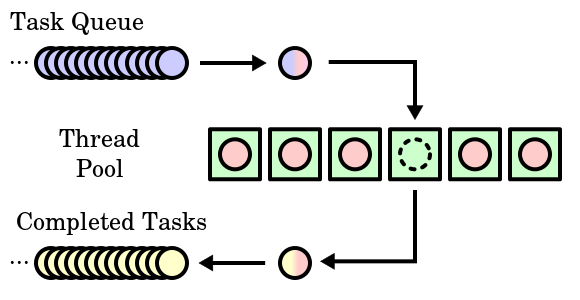
\includegraphics[width=\linewidth]{./pics/thread_pool.png}
  \caption{Thread Pool}
  \label{fig:Thread Pool}
\end{figure}

This diagram shows us the most basic and fundamental way to treat a process scheduling system. It's just a queue with tasks, inserted into a Thread Pool, which then picks one of the many tasks (or jobs), executes them, and sends them to the Complete Queue. Rinse and repeat.

\section{\underline{Specification and Analysis of the Software Requirements}}

\subsection{Requirements}

This software has a set of requirements that have to be met and covered in order to be held as working and complete, before it can be released for any pedagogical or personal usage. These specifications are separated into \textit{functional} and \textit{non-functional} requirements. The aim of the functional requirements is to describe what the software \textbf{should do}. Most of them aim at simplicity and ease of use of the application. The non-functional, on the other hand, try to provide a fast, extensible and stable experience to the user.

First, let's start with the analysis of the functional requirements. The software \textit{should}:

\begin{itemize}
\item \textit{Having a simple and readable user interface}. This means that all of the panels in the program should be easy to understand and differentiate between one another. Things like clear panel headlines, obvious execution patters, proper color coding of processes and commands, are a \textbf{must}. Each process should and will be assigned a priority either manually or automatically, but regardless, for each one, there should be a corresponding color that would give a general indication as to what that process's priority is. This goes hand in hand with how each process will be displayed in the different panels during execution. Because there will be commands that will create processes manually, each one should be clear, both with text and with color, what type of process is about to be created. In addition to the readability of the project, appropriate textual information should be given for each algorithm that is currently running. In the panel \textbf{Legend}, where all of this information will be held, a brief description of each action should be given, so that anyone who is executing an algorithm knows what is happening. Because this project will also be dynamically executing processes, it should also inform the user at each step what is happening. This means that the project should have a stable state at each moment and that the user knows it. This can be achieved through either labels or headings clearly shown in color at every moment.

\item \textit{Respond to all types of inputs}. One of the more complicated software aspects of this project is the responsiveness. Each process can executed for varying times, which means that the user might wait for one second or more, and although this is the normal behavior of the application, it should be made clear to the user that this is happening. With that, the user should be restricted to the commands and inputs he/she can do at any moment. The application is build to be light and fast, but it also has to handle every response from the \textit{UI}. This means that when an invalid character is submitted from the keyboard, the program should not be affected by it and should continue working. When a valid character is sent, the affects of that should also be made clear and responsive. Thus robustness is ensured for all users.

\item \textit{Be able to compare and analyze produced data}. Because this project has a purpose to evaluate and compare different algorithms, it should be made easy to have a set of saved \textit{already executed} processes and what their evaluation is. Thus, for each execution, every time and algorithm is executed, it should be saved for further evaluation and should be made easily readable by anyone. Then the last 10 executions and their summaries should be put on the screen when the user enters the appropriate command and wants to see and compare them. Finally, these summaries should be saved to a text file so that they can be separately analyzed if needed. Although only the last 10 executions will be shown, all of the previously run algorithms should be saved no matter what.
\end{itemize}

And here are some of the non-functional requirements. They focus on usability, efficiency, quality, speed, etc. These things focus on \textbf{how} the software \textit{should}:

\begin{itemize}
\item \textit{Create completely random processes}. Each process can either be created with a \textit{pre-defined} priority, or with an automatically set one (i.e. on a random principle). The processes that are randomly generated should be properly distributed and should not follow a pattern in any way. The need for such a requirement ensures that there are no hidden rules or patterns that would disrupt the evaluations and comparisons later on. That is why there has to be a proper distribution of processes with their values. For each process, the \code{ID} should be randomly generated to be a hexadecimal number with an even distribution between all processes, the \code{ttl} (time to live) should correspond to a \textit{Gaussian Distribution} with a predefined mean and standard deviation. The same should also apply to every \textit{IO} operation and their quantity.

\item \textit{Have high code quality}. Software craftsmanship is highly valued. It's expected that after the end of the project, maintenance and further improvements will be continually made, especially if the project is to be used for teaching purposes. If the code is not structured and prepared in such a way, that allows for further expansions and easy bug-fixing, then that would provide for a poor project life. This means that the code base should have correct comment sections, code documentation above each method, perfect separation of concerns, a valid architectural model that is followed to the end, diagrams that help understand the project and a list of future works to be done. If this is not met, then neither the original creator, nor any following contributor would want to maintain this software and any piece of code that is not regularly maintained, falls of the market and becomes useless.

\item \textit{Non-intrusive help from the User Interface}. It is very important that any form of help that comes from the system to be as inconspicuous as possible. User friendliness is achieved when the user thinks he/she have discovered something on their own. This should be done through layered error messages, that are generated on each step of processing, allowing for a decoupled, yet understandable explanation of the situation. In addition to this, all of the helper functions should have hints as to how to make the functionality of the project more approachable.
\end{itemize}

\underline{\textbf{Constraints}}

The application should \textbf{not} try to implement every algorithm for scheduling and have a \(1:1\) correspondence with real-life systems used in production. It should try to get as possible in order to do proper analysis and evaluation, without falling into the pit of meticulous pedantic, which are not worth implementing. This does not mean to restrict the number of algorithms, or to limit it to the most simple ones, but to put a realistic boundary on what should be expected from this product. A good mixture of complexity and quantity would fit the bill perfectly.

\subsection{\underline{Use cases}}

The use cases for this project are people who are interested in seeing how different process scheduling algorithms work underneath the hood and want to compare their abilities. For people who want to learn or get a better idea as to why systems are working the way they are, through running the application and looking at the source code, this project is a great place for research and learning.

use-case diagram

narrative diagram

pipeline diagram

activity diagram

\section{\underline{Design of the Software Solution}}

This software uses several algorithms and data-structures that play a key role in the whole inner-workings. Because the purpose of the project is to show how different algorithms affect the process execution of \textit{Real-Time} systems, we have to talk about each used algorithm and the accompanying data-structures.

But before we do that, we have to cover several structural decisions that have been made in order for the algorithm explanations to make sense.

Usually, in scheduling algorithms we have \code{PCB} blocks which hold references to the actual process, and through those blocks, we make decisions on which process should be executed next. Instead of doing this, because it adds another layer of complexity, not needed in this case, the role of a process and a PCB block is substituted with just a \code{process} class. It holds both the metadata found in PCBs and has the workings of processes. Thus, when in the text a reference is made to a process, a mental note should be made that it has a duality in it, for it holds two structures. The explanation of the \code{process} structure, as well as the other classes, can be found further down.

Another aspect that should be considered is that this project tries to imitate a \textit{Real-Time} system. This means that the scheduler has the notion of preemptive tasks and of \textit{IO} operations. Some of algorithms used are non-primitive and have been used in old \textit{batch systems} and \textit{interactive systems}. Thus, these algorithms have been tailored in order to work with a modern approach of building schedulers. When we refer to preemptive systems, it is meant that the OS decides when a process should be forced into a context-switch and when it should be taken from the \code{ready\_queue}. Also, Real Time systems do not wait for IO to end, thus they switch to the next ready process. For instance, the \textbf{FCFS} algorithm originally was used in non-preemptive batch systems, but in this project, each process is preempted upon requesting IO operations. Then, while waiting for that process to finish with IO, the next ready one is taken from the queue.

Having these distinctions made, we can then proceed to the algorithms and data-structures used.

\subsection{\underline{Algorithms and Data-structures}}

\subsubsection{\underline{FCFS}}

The \textbf{F}irst \textbf{C}ome \textbf{F}irst \textbf{S}erve algorithm is one of the easiest to understand and implement. It can be looked at from many different angles. \textbf{FCFS} can be seen as a \code{linked-list} or a \code{queue}, which just serves each incoming process to the CPU for execution. When a new process is created, it is put at the back of the \code{ready\_queue}. Then each process, one by one, is taken from the head of the queue and is given to the CPU for execution. It really depends on what type of system is running this scheduler, but in general, this algorithm, although easy, is not the most effective one to have. Because each process can take any time to finish, it can stall the whole system with its execution. For instance, if we were to have several processes and one is to be long in execution time, depending on their time of arrival, we can either quickly go through all of them, or we can wait for a long time.

In this project, the \textbf{FCFS} algorithm is created using a \code{vector} to hold all of the processes in sequential manner. At the start of the algorithm, we just take each next process for execution, wait for its time to live (\code{ttl}) and then we proceed to the next one in line. Because this project tries to imitate a \textit{Real-Time} system, we also check if each process will do an \textit{IO} operation. If so, the process is then sent to an \code{exec\_io} routine, and the next process is then taken. This means that the \code{done\_queue} will not be populated in the exact same order as the processes have been created in the \code{ready\_queue}, because of these \textit{IO} operations. Regardless, this still follows the \textbf{FCFS} pattern, and we can see that indeed, each process is taken from the head of the queue (technically vector).

\underline{\textbf{Evaluation}}

\textbf{FCFS} gives us a few benefits. First, it is very simple to implement and understand. From this standpoint, it's a great algorithm for small batch systems. But on the other hand, it doesn't scale well. It can stall if there is \textbf{no} preemption and a \textbf{convoy effect} might occur, which means that all other processes wait for the currently running one to finish. To summarize:

\begin{table}[H]
  \begin{tabularx}{\linewidth}{>{\parskip1ex}X@{\kern4\tabcolsep}>{\parskip1ex}X}
    \toprule
    \hfil\bfseries Pros & \hfil\bfseries Cons \\
    \cmidrule(r{3\tabcolsep}){1-1}\cmidrule(l{-\tabcolsep}){2-2}

    Easy to implement\par
    Easy to understand\par
    Works good for simple systems and batch systems\par

    &

    Can be slow\par
    Doesn't scale\par
    High risk of convoy effect\par
    System can stall if not preemptive\par
    Bad prediction for \textit{Waiting time} and \textit{Turnaround time} \\
    \bottomrule
  \end{tabularx}
  \caption{Pros and Cons of FCFS}
\end{table}

\

\underline{\textit{Example}}

Let's take a set of processes and see how they would hold under this algorithm. We generate 5 random processes.

\begin{table}[H]
  \begin{center}
    \label{tab:FCFS processes}
    \begin{tabular}{c|c}
      \toprule
      \textbf{Process ID} & \textbf{Time To Live} \\
      \midrule
      c37f & 2 \\
      e2fc & 5 \\
      792d & 3 \\
      0a35 & 5 \\
      3207 & 5 \\
      \bottomrule
    \end{tabular}
    \caption{FCFS processes table}
  \end{center}
\end{table}

From this, we can create the following \textbf{Gantt chart}.

\begin{ganttchart}[
  expand chart=\textwidth,
  hgrid={black}
  ]{1}{20}
  \gantttitle{FCFS}{20} \\
  \gantttitlelist{1,...,20}{1} \\
  \ganttbar[bar/.append style={fill=pr2}]{c37f}{1}{2} \\
  \ganttbar[bar/.append style={fill=pr3}]{e2fc}{3}{7} \\
  \ganttbar[bar/.append style={fill=pr2}]{792d}{8}{10} \\
  \ganttbar[bar/.append style={fill=pr3}]{0a35}{11}{15} \\
  \ganttbar[bar/.append style={fill=pr3}]{3207}{16}{20} \\
\end{ganttchart}

Then we can calculate the average \textbf{Waiting time} and \textbf{Turnaround time}.

\begin{table}[H]
  \begin{center}
    \label{tab:FCFS times}
    \begin{tabular}{c|c|c}
      \toprule
      \textbf{Process ID} & \textbf{Waiting time} & \textbf{Turnaround time} \\
      \midrule
      c37f & 0 & 2 \\
      e2fc & 2 & 5 \\
      792d & 7 & 3 \\
      0a35 & 10 & 5 \\
      3207 & 15 & 5 \\
      \bottomrule
      \toprule
      \textbf{Average} & \textbf{6.8} & \textbf{4} \\
    \end{tabular}
    \caption{FCFS times table}
  \end{center}
\end{table}

Of course this is a fairly simple example, because the processes do not take as long to execute, and we are also not taking into consideration the fact that these processes \textit{might} have some IO to do.

\subsubsection{\underline{SJF}}

The \textbf{S}hortest \textbf{J}ob \textbf{F}irst is another easy to understand, not so easy to implement algorithm. The SJF is an optimal algorithm, because it takes the greedy approach. It tries to finish all of the shortest processes first, which would cause the whole set of processes to finish as quick as possible. But there is a downside to this. This algorithm is not practically applicable, because it either relies on information beforehand for each process, or it has to do estimations for each upcoming process. Usually there is no way to know for how long a process will execute. In general, depending on what information we have, there are two ways to approach this algorithm.

\textbf{Note:} much like the FCFS, we also take into account the fact that we might have IO operations and we also preempt every process that does such actions.


\begin{itemize}
\item Method 1

In a perfect world, we would be graced with the knowledge of how long each job would. Thus, one way is to look in the \code{ready\_queue} and arrange the processes by their execution time in increasing manner (from smallest to largest). The shortest job will run first, then the second shortest one, and so on. Because each job has a \textit{pre-defined} execution time, which we take as a \textit{given}, based on that value, we sort the queue. This is the simpler approach because it only relies on information that is already given to us. It is important to note that this algorithm is a special case for a \textbf{PFJ} (Priority First Job) algorithm, because we are organizing the processes based on their execution time, which would be a form of a priority measurement.

\item Method 2

Continuing from \textit{Method 1}, we do not live in a perfect world and as we mentioned earlier, because we do not know before-hand what is the \textit{actual} time of execution for each process, we try to \textit{guess it}. This is done by predicting the next job execution time on the basis of the previous jobs. This so called \textit{exponential average} of the measured lengths of the previous jobs will provide a good guess as to what to expect. The \textit{exponential average} can be defined as follows: Let \scalebox{1.1}{\(t_{n}\)} be the length of the nth CPU burst. Let \scalebox{1.1}{\(\tau_{n+1}\)} be our prediction for the next CPU burst. Then \scalebox{1.1}{\(\forall \alpha,  0 \leq \alpha \leq 1\)}, we define
\end{itemize}

\begin{equation}
  \mathlarger{\tau_{n+1} = \alpha t_{n} + (1 - \alpha)\tau_{n}}
\end{equation}

Where \scalebox{1.1}{\(t_{n}\)} is the most recent information we have, \scalebox{1.1}{\(\tau_{n}\)} is the previous prediction, and \scalebox{1.1}{\(\alpha\)} is the weight of our past predictions. If \scalebox{1.1}{\(\alpha = 0 \rightarrow \tau_{n+1} = \tau_{n}\)}, which means that the previous history does not matter. If \scalebox{1.1}{\(\alpha = 1 \rightarrow \tau_{n+1} = t_{n}\)}, which means that only the most recent history matters. A good middle value (quite literally) can be to put \scalebox{1.1}{\(\alpha = {{}^{1}\!/_{2}}\)}. This way, both recent and past history have equal weight on the next \textit{exponential average}.

The expanded \textit{exponential average} formula looks like this

\begin{equation}
  \mathlarger{\tau_{n+1} = \alpha t_{n} + (1 - \alpha)\alpha t_{n - 1} + \dots + (1 - \alpha)^{j} \alpha t_{n - j} + \dots + (1 - \alpha)^{n + 1} \tau_{0}}
\end{equation}

Usually, \scalebox{1.1}{\(\alpha\)} is less than 1, thus each successive term has less and less weight than the previous one. By using this formula, we can then make an informed decision on how to execute each incoming process.

One thing that arises in this algorithm is why we must make a guess as to which process should be executed? Why is this happening? This type of guessing is done only here, while anywhere else, we do not need to make presumptions. The reason is that for all other algorithms, we either have a constant \code{TIME\_QUANTUM}, which is used to define each CPU burst (used in \textbf{Round-Robin Scheduling}), or we wait for the process to tell us if it's done or not (such as the case with \textbf{FCFS}). Here, however, we have to \textit{dynamically} specify the CPU burst time on each new process execution. This forces us to keep track of each execution time.

\underline{\textbf{Evaluation}}

\begin{table}[H]
  \begin{tabularx}{\linewidth}{>{\parskip1ex}X@{\kern4\tabcolsep}>{\parskip1ex}X}
    \toprule
    \hfil\bfseries Pros & \hfil\bfseries Cons \\
    \cmidrule(r{3\tabcolsep}){1-1}\cmidrule(l{-\tabcolsep}){2-2}

    Optimal\par
    A good academic exercise\par
    Can produce fast results\par

    &

    Somewhat difficult to implement\par
    Cannot be used in a real system\par
    Still might have a process that stalls \\
    \bottomrule
  \end{tabularx}
  \caption{Pros and Cons of SJF}
\end{table}

In this case we might think that FCFS is the better algorithm, since at least it has some real life value to it, but that's not the immediate case. Although we are dealing with a hypothetical algorithm here, it is still worth it to check what are the times for SJF. If we run an example, we would see that SJF has better waiting time for each process, where the turnaround time doesn't change. Thus, SJF yields better results on average that FCFS.

\underline{\textit{Example}}

Let's take again a set of processes and see how they would work. Then we can create the \textbf{Gantt chart}.

\begin{table}[H]
  \begin{center}
    \label{tab:SJF processes}
    \begin{tabular}{c|c}
      \toprule
      \textbf{Process ID} & \textbf{Time To Live} \\
      \midrule
      9479 & 2 \\
      7470 & 3 \\
      2b62 & 4 \\
      047c & 4 \\
      d19c & 7 \\
      \bottomrule
    \end{tabular}
    \caption{SJF processes table}
  \end{center}
\end{table}

\begin{ganttchart}[
  expand chart=\textwidth,
  hgrid={black}
  ]{1}{20}
  \gantttitle{SJF}{20} \\
  \gantttitlelist{1,...,20}{1} \\
  \ganttbar[bar/.append style={fill=pr1}]{9479}{1}{2} \\
  \ganttbar[bar/.append style={fill=pr3}]{7470}{3}{5} \\
  \ganttbar[bar/.append style={fill=pr3}]{2b62}{6}{9} \\
  \ganttbar[bar/.append style={fill=pr3}]{047c}{10}{13} \\
  \ganttbar[bar/.append style={fill=pr4}]{d19c}{14}{20} \\
\end{ganttchart}

Then we can calculate the average \textbf{Waiting time} and \textbf{Turnaround time}.

\begin{table}[H]
  \begin{center}
    \label{tab:SJF times}
    \begin{tabular}{c|c|c}
      \toprule
      \textbf{Process ID} & \textbf{Waiting time} & \textbf{Turnaround time} \\
      \midrule
      9479 & 0 & 2 \\
      7470 & 2 & 3 \\
      2b62 & 5 & 4 \\
      047c & 9 & 4 \\
      d19c & 13 & 7 \\
      \bottomrule
      \toprule
      \textbf{Average} & \textbf{5.8} & \textbf{4} \\
    \end{tabular}
    \caption{SJF times table}
  \end{center}
\end{table}

\subsubsection{\underline{Round-Robin}}

\subsubsection{\underline{Priority Job First}}

\subsubsection{\underline{Completely Fair Scheduling}}

\subsubsection{\underline{Normal and Even Distributions for Processes}}

\subsubsection{\underline{Data-structures}}

Because we are working with a lot of different types of classes, which interact heavily during every procedure, it's a good idea to see what each object does and in what type of structure does it integrate with. The classes that are involved with the process scheduling algorithms are as follows:

\begin{itemize}
\item \code{process} \\
  This class holds the data for each process. Instead of using a separate \code{PCB} block, which points to another \code{process} object, the project has been simplified for ease of use, thus it incorporates both these classes into one. The \code{process} class keeps track of its different statistics, which are then summarized in the end for the final evaluation. Each process has \textit{pre-defined} priority, or it can be evaluated upon creation, based on a normal distribution. Each process holds
  \begin{itemize}
  \item \textit{time to live} - \code{ttl}. The time each process it takes to execute completely.
  \item \textit{time of submission} - \code{tos}. The time at which the process starts executing.
  \item \textit{time of completion} - \code{toc}. The time at which the process finishes executing.
  \item \textit{turnaround time} - \code{tat}. The time between the time of submission and time of completion plus any \textit{IO} execution.
  \item \textit{waiting time} - \code{wait\_t}. The time a process spends in the \code{read\_queue} and is \textbf{not} executing.
  \item \textit{priority} - \code{prty}. The priority each process is assigned based on its execution time, or predefined from the start.
  \item \textit{IO operations} - \code{ioops}. The set of IO operations each process has.
  \item \textit{process id} - \code{id}. The unique ID that each process has.
  \end{itemize}
  In addition, this class also holds the data about its distribution, as specified in the previous section, in the for of constants.
\item \code{pool} \\
  This class used as a global pool, holding all of the different processes in their different states. Thus, there are \textit{queues} for \textbf{waiting processes}, \textbf{ready processes} and \textbf{done processes}. The pool itself is used as a general interface towards each process and its current structure. Because of this, it is much easier to perform operations on these queues, such as checking if they are empty, or clearing them, or even evaluating each process in a specific queue.
\item \code{scheduler}
  The scheduler is the structure that is responsible for controlling each executing algorithm. It interacts with the pool of processes, and executes them on the specified procedure. In addition to this, the scheduler also calculates \textit{both} the current and final \textbf{average waiting time} and \textbf{average turnaround time} of each algorithm, based on the passed processes. The class also specifies additional constants, like an \code{ALPHA} value for future predictions, and \code{TIME\_QUANTUM} for equal process execution. \\
  The general steps of execution are like this:
  \begin{center}
    \begin{lstlisting}
START:
    take_first_process
    check for io
    dispetcher:
    \end{lstlisting}
  \end{center}
\item \code{dispatcher}
\item \code{scheduler}
\end{itemize}

\subsubsection{\underline{User Interface}}

\subsubsection{\underline{Software Architecture}}

The Software Architecture of the project can be seen as one of the following: \textit{Monolithic}, \textit{Event-driven}, or \textit{Procedural}. If we look at the project as a \textit{Monolithic}, we can say that it encapsulates itself into a \textit{single-tiered} software application in which the user interface and data access code are combined into a single program from a single platform. A monolithic application is self-contained, and independent from other computing applications. The design philosophy is that the application is responsible not just for a particular task, but can perform every step needed to complete a particular function. On the other hand, were we to look at it through the perspective of the \textit{Event-driven} design, we can see how it follows a pattern promoting the production, detection, consumption of, and reaction to events. An \textit{event} can be defined as \textit{"a significant change in state"}. For example, when a \textbf{process} \code{ttl} is completely done, it changes state from \code{RUNNING} to \code{DONE}. And again, if we are to look at the project from the standpoint of a \textit{Procedural} system, we would see that it follows a certain set of rules, which in the end, produce an output that can be interpreted and evaluated for further work. As an example, we would be able to see how the \textbf{SJF} algorithm performs under long processes.

\subsubsection{\underline{Security Features}}

\section{\underline{Implementation}}

This software is developed entirely with the \code{C++} programming language. All of the implementation uses the \code{C++ 11} standard (and up). The \code{C++ 11} standard and all of its follow-up additions, all the way up to \code{C++ 20}, have great benefits to creating modern, safe, and easy to manage software. Many functionalities introduced since \code{C++ 11} have been used to create this project. Most noticeably, the use of lambda functions, collection manipulators, threads and mutexes, and many more, play a key role.

In addition to this, the famous library \code{ncurses} is used in order to make working with terminal emulators easier. \code{ncurses} provides an \code{API} for manipulating the graphics and output of the terminal. Since this is an application, based on working with a terminal emulator, such a library would be of great help. The specific terminal that was used to test and run the application is \code{xterm}, but this was also tested on \code{gnome-terminal}.

The operating system used to create the software is \code{Arch Linux}, with additional testing environment under \code{Fedora 29}.

\section{\underline{Testing}}

\section{\underline{Result and Conclusion}}

\section{\underline{References}}

\end{document}